\documentclass[noauthor,nooutcomes,hints]{ximera}

\graphicspath{  
{./}
{./whoAreYou/}
{./drawingWithTheTurtle/}
{./bisectionMethod/}
{./circles/}
{./anglesAndRightTriangles/}
{./lawOfSines/}
{./lawOfCosines/}
{./plotter/}
{./staircases/}
{./pitch/}
{./qualityControl/}
{./symmetry/}
{./nGonBlock/}
}


%% page layout
\usepackage[cm,headings]{fullpage}
\raggedright
\setlength\headheight{13.6pt}


%% fonts
\usepackage{euler}

\usepackage{FiraMono}
\renewcommand\familydefault{\ttdefault} 
\usepackage[defaultmathsizes]{mathastext}
\usepackage[htt]{hyphenat}

\usepackage[T1]{fontenc}
\usepackage[scaled=1]{FiraSans}

%\usepackage{wedn}
\usepackage{pbsi} %% Answer font


\usepackage{cancel} %% strike through in pitch/pitch.tex


%% \usepackage{ulem} %% 
%% \renewcommand{\ULthickness}{2pt}% changes underline thickness

\tikzset{>=stealth}

\usepackage{adjustbox}

\setcounter{titlenumber}{-1}

%% journal style
\makeatletter
\newcommand\journalstyle{%
  \def\activitystyle{activity-chapter}
  \def\maketitle{%
    \addtocounter{titlenumber}{1}%
                {\flushleft\small\sffamily\bfseries\@pretitle\par\vspace{-1.5em}}%
                {\flushleft\LARGE\sffamily\bfseries\thetitlenumber\hspace{1em}\@title \par }%
                {\vskip .6em\noindent\textit\theabstract\setcounter{question}{0}\setcounter{sectiontitlenumber}{0}}%
                    \par\vspace{2em}
                    \phantomsection\addcontentsline{toc}{section}{\thetitlenumber\hspace{1em}\textbf{\@title}}%
                     }}
\makeatother



%% thm like environments
\let\question\relax
\let\endquestion\relax

\newtheoremstyle{QuestionStyle}{\topsep}{\topsep}%%% space between body and thm
		{}                      %%% Thm body font
		{}                              %%% Indent amount (empty = no indent)
		{\bfseries}            %%% Thm head font
		{)}                              %%% Punctuation after thm head
		{ }                           %%% Space after thm head
		{\thmnumber{#2}\thmnote{ \bfseries(#3)}}%%% Thm head spec
\theoremstyle{QuestionStyle}
\newtheorem{question}{}



\let\freeResponse\relax
\let\endfreeResponse\relax

%% \newtheoremstyle{ResponseStyle}{\topsep}{\topsep}%%% space between body and thm
%% 		{\wedn\bfseries}                      %%% Thm body font
%% 		{}                              %%% Indent amount (empty = no indent)
%% 		{\wedn\bfseries}            %%% Thm head font
%% 		{}                              %%% Punctuation after thm head
%% 		{3ex}                           %%% Space after thm head
%% 		{\underline{\underline{\thmname{#1}}}}%%% Thm head spec
%% \theoremstyle{ResponseStyle}

\usepackage[tikz]{mdframed}
\mdfdefinestyle{ResponseStyle}{leftmargin=1cm,linecolor=black,roundcorner=5pt,
, font=\bsifamily,}%font=\wedn\bfseries\upshape,}


\ifhandout
\NewEnviron{freeResponse}{}
\else
%\newtheorem{freeResponse}{Response:}
\newenvironment{freeResponse}{\begin{mdframed}[style=ResponseStyle]}{\end{mdframed}}
\fi



%% attempting to automate outcomes.

%% \newwrite\outcomefile
%%   \immediate\openout\outcomefile=\jobname.oc
%% \renewcommand{\outcome}[1]{\edef\theoutcomes{\theoutcomes #1~}%
%% \immediate\write\outcomefile{\unexpanded{\outcome}{#1}}}

%% \newcommand{\outcomelist}{\begin{itemize}\theoutcomes\end{itemize}}

%% \NewEnviron{listOutcomes}{\small\sffamily
%% After answering the following questions, students should be able to:
%% \begin{itemize}
%% \BODY
%% \end{itemize}
%% }
\usepackage[tikz]{mdframed}
\mdfdefinestyle{OutcomeStyle}{leftmargin=2cm,rightmargin=2cm,linecolor=black,roundcorner=5pt,
, font=\small\sffamily,}%font=\wedn\bfseries\upshape,}
\newenvironment{listOutcomes}{\begin{mdframed}[style=OutcomeStyle]After answering the following questions, students should be able to:\begin{itemize}}{\end{itemize}\end{mdframed}}



%% my commands

\newcommand{\snap}{{\bfseries\itshape\textsf{Snap!}}}
\newcommand{\flavor}{\link[\snap]{https://snap.berkeley.edu/}}
\newcommand{\mooculus}{\textsf{\textbf{MOOC}\textnormal{\textsf{ULUS}}}}


\usepackage{tkz-euclide}
\tikzstyle geometryDiagrams=[rounded corners=.5pt,ultra thick,color=black]
\colorlet{penColor}{black} % Color of a curve in a plot



\ifhandout\newcommand{\mynewpage}{\newpage}\else\newcommand{\mynewpage}{}\fi


\title{Symmetries of the regular triangle}

\author{Bart Snapp}

\begin{document}
\begin{abstract}
  We explore the symmetries of the regular triangle.
\end{abstract}
\maketitle

\begin{listOutcomes}
\item Witness the symmetries of the regular triangle.
\item Describe symmetries of the regular triangle.
\item Think of the symmetries of the regular triangle as functions.
\item Compose symmetries and use \snap\ to show the result.
\item Use the algebra of symmetries to understand a composition of
  symmetries.
\end{listOutcomes}


A \textbf{regular} $n$-gon is a $n$-sided shape where all the side
lengths are the same and all the angles are the same. As a gesture of
friendship, I present you with the \snap\ block
\raisebox{-.4\height}{
\includegraphics{regularNGonBlockBLANK.png}}. To
use this block, input a number of sides, $n$, for the first blank and
an angle $r$ for the second. When you do this,
\raisebox{-.4\height}{
\includegraphics{regularNGonBlockBLANK.png}}
draws a regular $n$-gon where pressing:
\begin{itemize}
\item \textbf{SPACE-BAR} toggles the colors of the $n$-gon.
\item \textbf{R} rotates the $n$-gon $r$ degrees.
\item \textbf{F} flips the $n$-gon across a central vertical line.
\end{itemize}



\mynewpage


\begin{question}
  The \textbf{symmetries} of the regular triangle are those that
  \textbf{leave it unchanged}. So for example, here is a symmetry of
  the regular triangle:
  \[
  \raisebox{-.4\height}{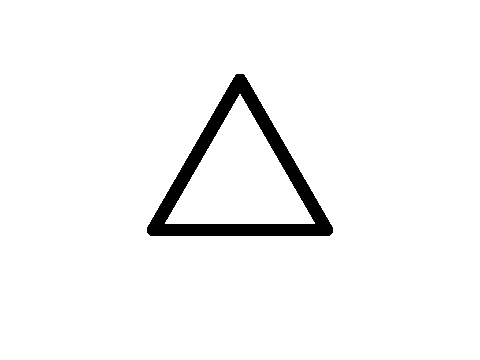
\includegraphics[width=2.5in]{blackSymTri.png}}\resizebox{.7in}{!}{$\mapsto$} \raisebox{-.4\height}{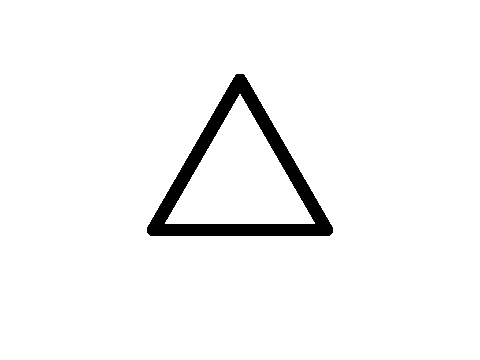
\includegraphics[width=2.5in]{blackSymTri.png}}
  \]
  You may think nothing happened above, because the triangle is
  unchanged, but you would be wrong.  To WITNESS symmetries, we must
  color-in the sides of the triangle. For example once I color in the
  sides, we see that the symmetry above is acutally:
  \[
  \raisebox{-.4\height}{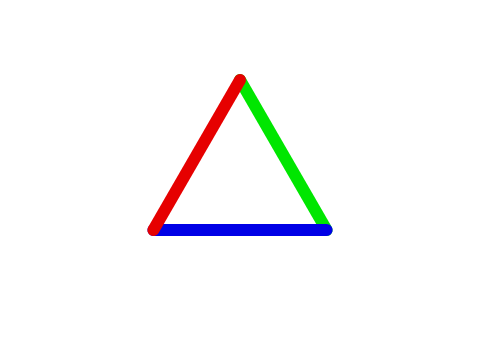
\includegraphics[width=2.5in]{eTri.png}}\resizebox{.7in}{!}{$\mapsto$} \raisebox{-.4\height}{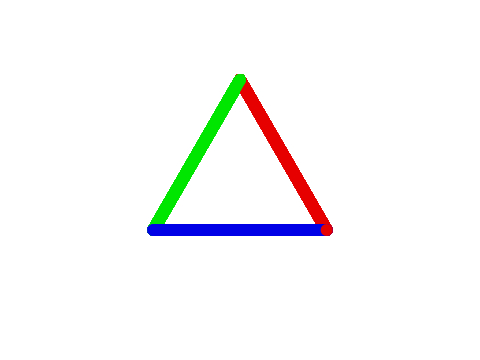
\includegraphics[width=2.5in]{rfTri.png}}
  \]
  While the colors change, the ACTUAL TRIANGLE is \textbf{unchanged}.
  \begin{enumerate}
  \item How MANY symmetries does the equilateral triangle have?
  \item Use
    \raisebox{-.4\height}{
\includegraphics{regularNGonBlockBLANK.png}}
    to make STAGES for (the output of) each symmetry of the regular
    triangle.
  \end{enumerate}
  \begin{freeResponse}
    \begin{enumerate}
    \item There are SIX symmetries of the regular triangle.
    \item Here they are:
    \begin{enumerate}
    \item $\raisebox{-.4\height}{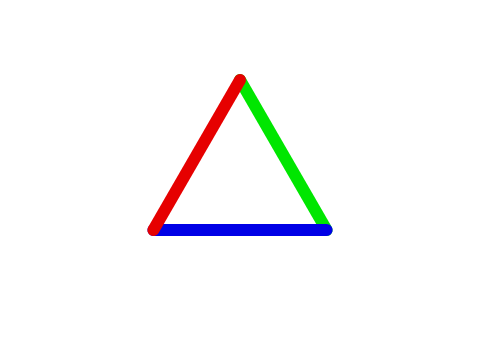
\includegraphics[width=2in]{eTri.png}}\resizebox{.5in}{!}{$\mapsto$} \raisebox{-.4\height}{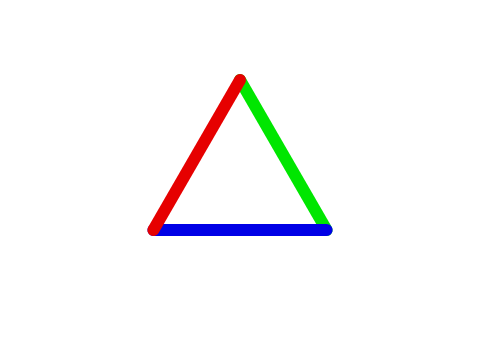
\includegraphics[width=2in]{eTri.png}}$
    \item $\raisebox{-.4\height}{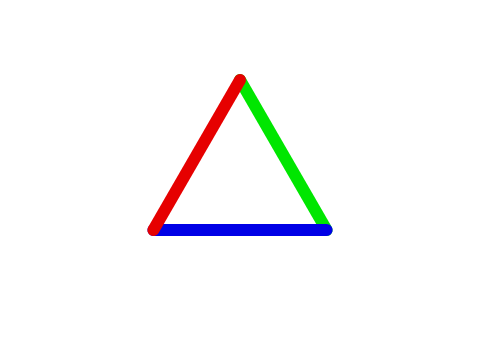
\includegraphics[width=2in]{eTri.png}}\resizebox{.5in}{!}{$\mapsto$} \raisebox{-.4\height}{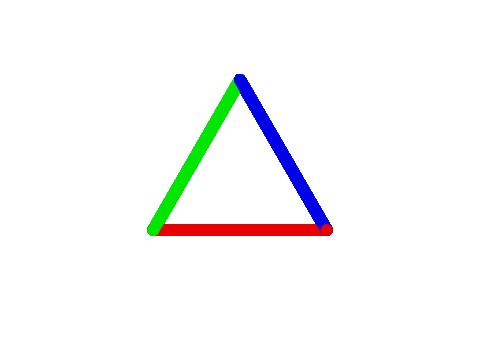
\includegraphics[width=2in]{rTri.png}}$
    \item $\raisebox{-.4\height}{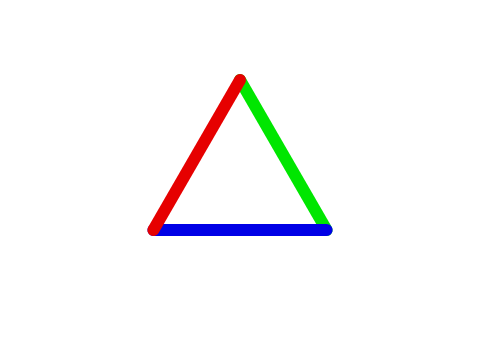
\includegraphics[width=2in]{eTri.png}}\resizebox{.5in}{!}{$\mapsto$} \raisebox{-.4\height}{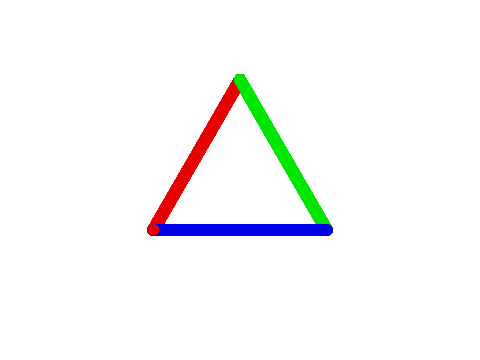
\includegraphics[width=2in]{r2Tri.png}}$
    \item $\raisebox{-.4\height}{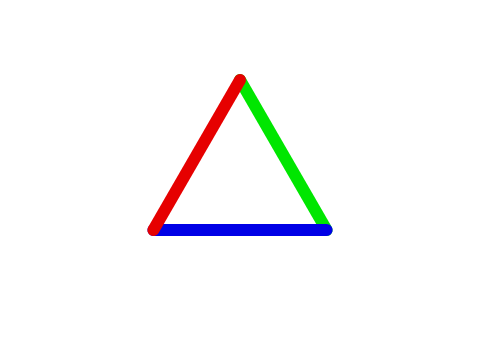
\includegraphics[width=2in]{eTri.png}}\resizebox{.5in}{!}{$\mapsto$} \raisebox{-.4\height}{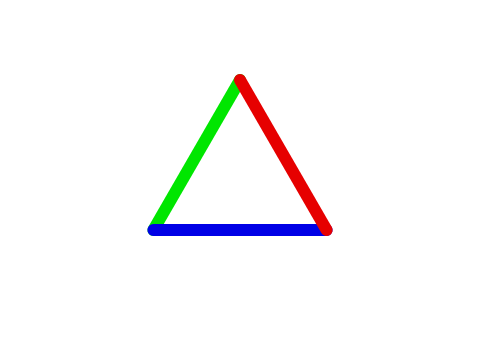
\includegraphics[width=2in]{fTri.png}}$
    \item $\raisebox{-.4\height}{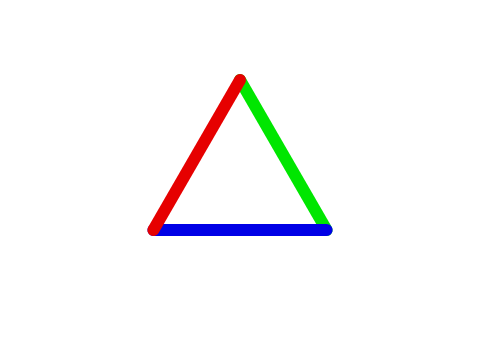
\includegraphics[width=2in]{eTri.png}}\resizebox{.5in}{!}{$\mapsto$} \raisebox{-.4\height}{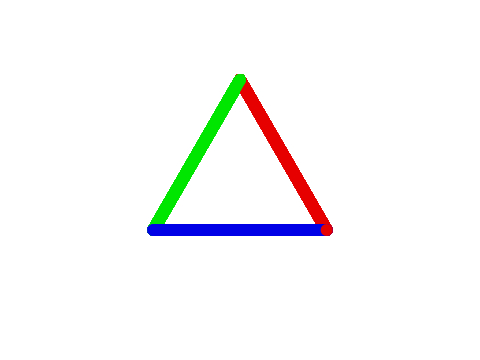
\includegraphics[width=2in]{rfTri.png}}$
    \item $\raisebox{-.4\height}{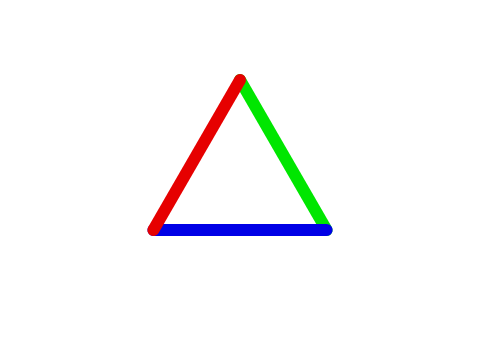
\includegraphics[width=2in]{eTri.png}}\resizebox{.5in}{!}{$\mapsto$} \raisebox{-.4\height}{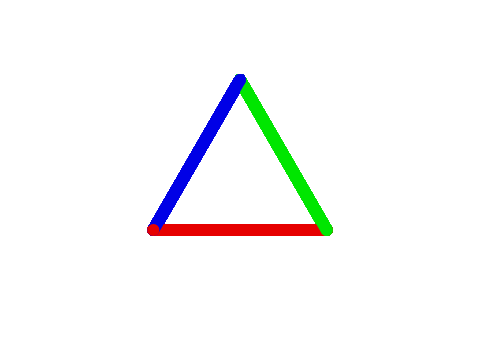
\includegraphics[width=2in]{r2fTri.png}}$
    \end{enumerate}
    \end{enumerate}
  \end{freeResponse}
\end{question}
\mynewpage

\begin{question}
  Let $e$ be the do-nothing symmetry, $r$ be a clockwise $120^\circ$
  rotation about the center of the triangle, and $f$ be a flip across
  a vertical line down the middle of the triangle. When $e$ is
  applied, the triangle looks like this:
  \[
  \raisebox{-.4\height}{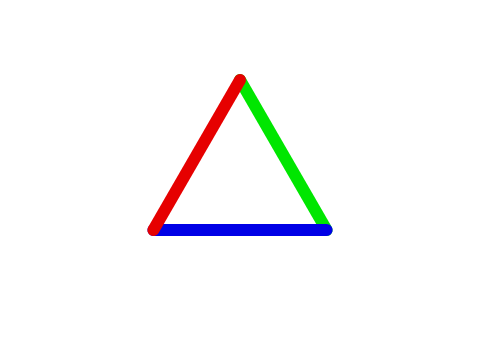
\includegraphics[width=2.5in]{eTri.png}}\resizebox{.7in}{!}{$\overset{\scriptscriptstyle e}{\mapsto}$} \raisebox{-.4\height}{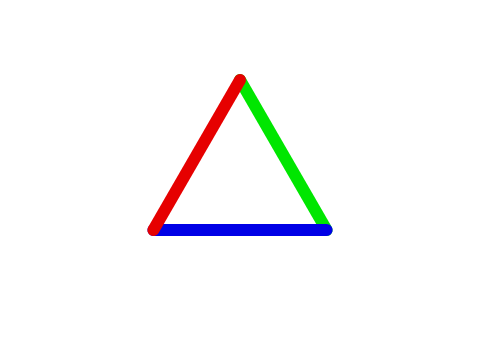
\includegraphics[width=2.5in]{eTri.png}}
  \]
  Display the result of applying the following functions
  (actions/transformations) to your triangle:
  \begin{enumerate}
  \item $rf$
  \item $fr$
  \item $r^2 f$
  \item $f r^2$
  \end{enumerate}
  In each case, show off your work by displaying your STAGE.
  \begin{hint}
    Note, when looking at something like $rf$, first we flip the
    triangle, then we rotate it. Just like if $f(x) = x^2$ and $g(x) =
    2x+1$, then when we look at $(f\circ g)(x)$ we apply $g$ first,
    and $f$ second.
  \end{hint}
  \begin{freeResponse}
    \begin{enumerate}
    \item For $rf$ I have
      \[
      \raisebox{-.4\height}{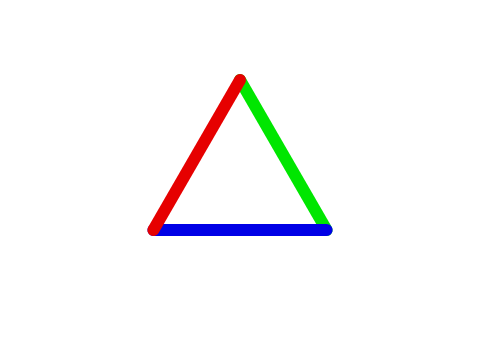
\includegraphics[width=2.5in]{eTri.png}}\resizebox{.7in}{!}{$\overset{\scriptscriptstyle rf}{\mapsto}$} \raisebox{-.4\height}{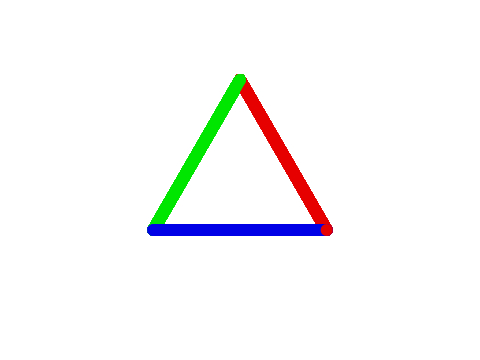
\includegraphics[width=2.5in]{rfTri.png}}
      \]
    \item For $fr$ I have
      \[
      \raisebox{-.4\height}{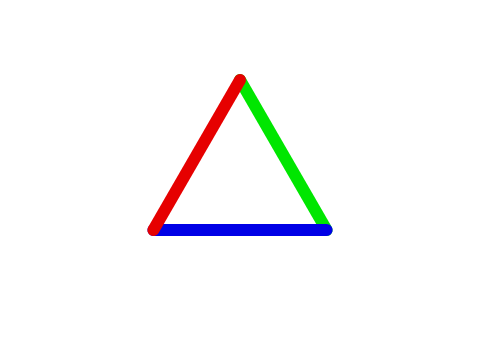
\includegraphics[width=2.5in]{eTri.png}}\resizebox{.7in}{!}{$\overset{\scriptscriptstyle fr}{\mapsto}$} \raisebox{-.4\height}{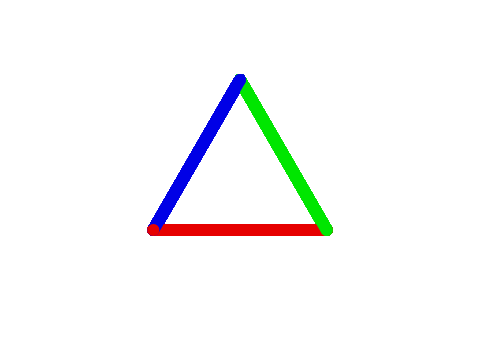
\includegraphics[width=2.5in]{r2fTri.png}}
      \]
    \item For $r^2f$ I have
      \[
      \raisebox{-.4\height}{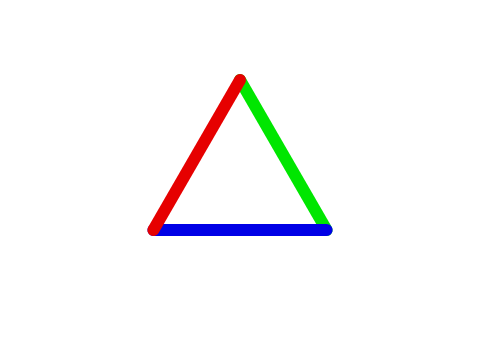
\includegraphics[width=2.5in]{eTri.png}}\resizebox{.7in}{!}{$\overset{\scriptscriptstyle r^2f}{\mapsto}$} \raisebox{-.4\height}{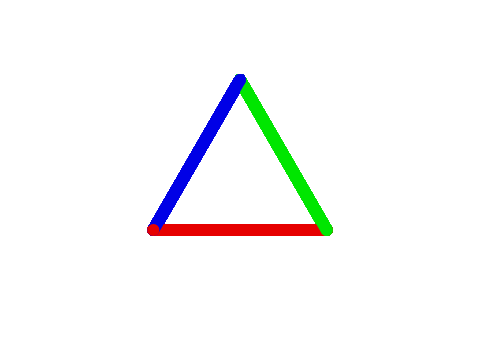
\includegraphics[width=2.5in]{r2fTri.png}}
      \]
    \item For $fr^2$ I have
      \[
      \raisebox{-.4\height}{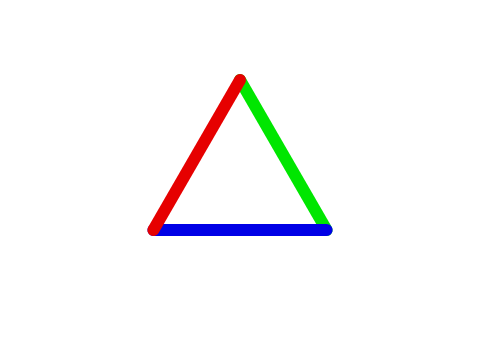
\includegraphics[width=2.5in]{eTri.png}}\resizebox{.7in}{!}{$\overset{\scriptscriptstyle  fr^2}{\mapsto}$} \raisebox{-.4\height}{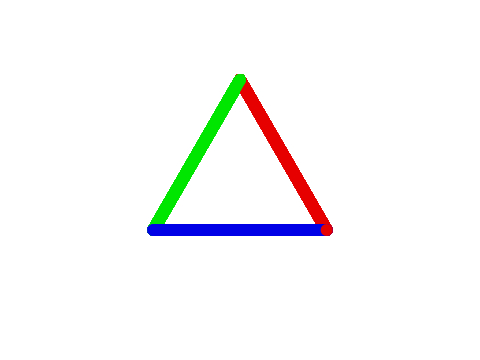
\includegraphics[width=2.5in]{rfTri.png}}
      \]
    \end{enumerate}
    \end{freeResponse}
\end{question}
\mynewpage


\begin{question}
  Do you remember the MULTIPLICATION TABLES? We can make a similar
  table for the symmetries of the regular triangle. Here, I've
  started it for you:
  \[
  \begin{array}{|c||c|c|c|c|c|c|}
    \hline
      & e & r & r^2 & f & rf & r^2f\\ \hline\hline
    e & e & r & r^2 & f & rf & r^2f\\ \hline
    r & r & r^2 & \color{red}r^3 & rf & r^2f & \color{red}r^3f\\ \hline
    r^2 & r^2 & \color{red}r^3 & \color{red}r^4 & r^2f & \color{red}r^3f &\color{red} r^4f\\ \hline
    f  & f & \color{red}fr & \color{red}fr^2 & \color{red}f^2 & \color{red}frf & \color{red}fr^2f\\ \hline
    rf & rf & \color{red}rfr & \color{red}rfr^2 & \color{red}rf^2 & \color{red}rfrf & \color{red}rfr^2f\\ \hline
    r^2f & r^2f & \color{red}r^2fr & \color{red}r^2fr^2 & \color{red}r^2f^2 &\color{red} r^2frf &\color{red} r^2fr^2f\\ \hline
  \end{array}
  \]
  Each of the symmetries in red is actually equal to one of the
  symmetries in top row (or left-most column)
  \[
  e,\quad r,\quad r^2,\quad f,\quad rf,\quad r^2f
  \]
  where $e$ is the ``do-nothing'' symmetry.
  \begin{enumerate}
    \item EXPRESS each of the red symmetries as one of
      $e,r,r^2,f,rf,r^2f$ and UPDATE the table with these values.
    \item Use your table to express
      \[
      fr^5fr^2
      \]
      as one of $e,r,r^2,f,rf,r^2f$.
  \end{enumerate}
  \begin{freeResponse}
      \begin{enumerate}
      \item
      Here is my updated table:
       \[
  \begin{array}{|c||c|c|c|c|c|c|}
    \hline
    & e & r & r^2 & f & rf & r^2f\\ \hline\hline
    e & e & r & r^2 & f & rf & r^2f\\ \hline
    r & r & r^2 & e & rf & r^2f & f\\ \hline
    r^2 & r^2 & e & r & r^2f & f &rf\\ \hline
    f  & f & r^2f & rf & e & r^2 & r\\ \hline
    rf & rf & f & r^2f & r & e & r^2\\ \hline
    r^2f & r^2f & rf & f & r^2 & r & e\\ \hline
  \end{array}
  \]
\item Using the table I see
  \begin{align*}
    fr(frfrrf) &= r^2f(frfr^2f)\\
    &= fr^2f\\
    &=r.
  \end{align*}
    \end{enumerate}
  \end{freeResponse}
\end{question}
\end{document}
